\documentclass{article}
\usepackage[final]{nips_2017}
\usepackage[utf8]{inputenc} % allow utf-8 input
\usepackage[T1]{fontenc}    % use 8-bit T1 fonts
\usepackage{hyperref}       % hyperlinks
\usepackage{url}            % simple URL typesetting
\usepackage{booktabs}       % professional-quality tables
\usepackage{amsfonts}       % blackboard math symbols
\usepackage{nicefrac}       % compact symbols for 1/2, etc.
\usepackage{microtype}      % microtypography
\usepackage{graphicx}
\usepackage{subcaption}
\title{Spoken Command Recognition}

\author{
  Thomas Karpati \\
  Department of Computer Science\\
  Stanford University\\
  \texttt{tkarpati@stanford.edu} \\
  %% examples of more authors
  %% \And
  %% Coauthor \\
  %% Affiliation \\
  %% Address \\
  %% \texttt{email} \\
  %% \AND
  %% Coauthor \\
  %% Affiliation \\
  %% Address \\
  %% \texttt{email} \\
  %% \And
  %% Coauthor \\
  %% Affiliation \\
  %% Address \\
  %% \texttt{email} \\
  %% \And
  %% Coauthor \\
  %% Affiliation \\
  %% Address \\
  %% \texttt{email} \\
}

\begin{document}
% \nipsfinalcopy is no longer used

\begin{center}

\includegraphics[width=3cm, height=0.7cm]{CS230}
\end{center}

\maketitle

\begin{abstract}
  Interactions with agents in the world has been increasing using voice
  commands. This allows users to interact without the use of a
  terminal input such as when they are not in close proximity, are
  otherwise physically occupied, or enable users such as children who
  are illiterate and cannot use standard computing interaces which
  would require the ability to read. In the simple case such an agent
  would need to be able to recognize basic commands to perform
  tasks. One of the preprocessing steps which is common for speech
  recognition is the use of the spectrograph. This operation converts
  the single dimension of an audio saple to a two dimensional
  representation of the audio waveform through a basis
  transformation. This representation can be processed as a two
  dimensional image to extract features before passing this to a
  sequential model. 
\end{abstract}

\section{Introduction}
Speech recognition is allowing more accessible interactions with
agents. Deep learning systems have allowed for improved speech
recognition accuracy through sequential models. Often the inputs to
these sequential models is the spectrogram representation of an audio
waveform. The spectrogram is a representation which converts the time
domain audio waveform into a multidimensional basis space for segments
of time within a sliding window. The result of this is a
multidimensional representation of the audio waveform during a
specified period of time. As these are accumulated over time, this can
be seen as a two dimensional representation of the audio waveform. Our
alogrithm explores applying two dimmensional network architectures to
a traditional sequential model for speech recognition processing. 



TODO: Remove
Explain the problem and why it is important. Discuss your motivation for pursuing this
problem. Give some background if necessary. Clearly state what the input and output
is. Be very explicit: “The input to our algorithm is an {image, amplitude, patient age,
rainfall measurements, grayscale video, etc.}. We then use a {SVM, neural network, linear
regression, etc.} to output a predicted {age, stock price, cancer type, music genre, etc.}.”
This is very important since different teams have different inputs/outputs spanning different
application domains. Being explicit about this makes it easier for readers. If you are using
your project for multiple classes, add a paragraph explaining which components of the
project were used for each class.

\section{Related work}
There are several approaches to the speech recognition
problem. Dominant approaches involve use of recurrent networks which
take the sequential nature of the audio as it progresses through time
into account. These vary from those with simple recurrent cells to
larger more comples bi-directional recurrent cells that process large
segments of time at once. Other approaches to the command recognition
problem involve use of both 1D and 2D convolutional networks as will
as somple fully connected dense networks over the spectrogram of the
data.

Both of these appoaches have their advanatages and drawbacks. The use
of the fully connected dense and two dimensional convolutional
networks can extract significant features across the entire space of
the input to the network by using the entire time and frequency
information available. The 2D convolutional network is able to extract
features from both across time and across frequencies by applying
network structures from image processing to the spectrogram. This
approach does ignore the sequential nature of the data (but can take this
into account by the relative weights of the connections to different
parts of the spectrogram) however the exact position of the utterance
in question needs to known so that the utterance can be located
properly within the time frame that is being looked at. The assumption
here is that the time of the utterance is known.

The recurrent networks take the sequential nature of speech into
account. These networks have shown to be highly effective in speech
recognition, and typically use the spectrogram as the input feature
transformation to the input of the network. Effective speech
recognition systems will typically also employ bidirectional recurrent
cells for encoding the speech data. The drawback here is that
bidirectional networks will impact the latency for command
detection. While effective for speech-to-text or translation domains,
keyword and command recognition system are latency sensitive, and thus
the bidirectional nature of these recurrent networks are
impractical. Also, systems which implement 1D convolution before the
recurrent cells, while taking the frequency domain into account, do
not fully allow for convolution across the frequencies. Even systems
that only convolve in two dimensions may not be taking invariance into
account in the input waveforms.

We seek to overcome the limitations of either of these approaches by
both implementing the convolutional approach and using this to feed
into a forward only recurrent layer. Following from image processing
convolutional network, we extend these architectures with multiple two
dimensional (time and frequency domain) convolutions followed by a max
pooling layer to add invariance and reduce the inputs to the following
layers.

TODO: Simple diagrams of the networks.

TODO: Cite related work here.

TODO: Provide current state of the art accuracy from related work

TODO: Remove
You should find existing papers, group them into categories based on their approaches,
and discuss their strengths and weaknesses, as well as how they are similar to and differ
from your work. In your opinion, which approaches were clever/good? What is the stateof-the-art?
Do most people perform the task by hand? You should aim to have at least
5 references in the related work. Include previous attempts by others at your problem,
previous technical methods, or previous learning algorithms. Google Scholar is very useful
for this: https://scholar.google.com/ (you can click “cite” and it generates MLA, APA,
BibTeX, etc.)

\section{Dataset and Features}
To evaluate models for spoken command recognition, the dataset used
was provided for the Kaggle TensorFlow speech recognition
challenge (TODO: CITE HERE)[2][3]. This dataset contains 10 labelled commands
which are ``yes'', ``no'', ``up'', ``down'', ``left'', ``right'', ``on'', ``off'',
``stop'', and ``go''. In addition to these, the dataset is augmented with
two additional classes which are “unknown” and silence. The “unknown”
class contains other utterances that are not the commands that we are
trying to catagorize. The silence class corresponds to no
utterance, but rather background noise. The input data is provided as
audio clips in WAV format sampled at 16Khz. This data set therefore
maps an audio file to 12 possible classes. The audio provided is all
approximately 1 sec in duration, with some slight variation in
length. The dataset contains 64,727 audio samples. With the samples
are also provided lists of samples for both validation and test set
splitting. There are 6835 valiation samples and 6798 test samples
provided. The remaining of the 64,727 samples are used for training.

The entire data set comprises 30 possible spoken commands in
approximately equal distribution. Of these, only 10 are commands that
are to be differentiated. The remaining 20 are other words that are
spoken which get pooled into the ``unknown'' class and are not
differentiated.

The 64,727 audio samples were preprocessed. For each sample, if the
sample belonged to the 10 classes that we are interested in, they were
labeled with that class, otherwise they were labeled with the
``unknown'' class. If the sample was background noise, it was labeled
with the ``silence'' class. After the samples were re-binned into the
classes that we are interested in, they were all converted to a common
size. Most samples are of 1 second in duration at 16Khz, or 16,000
samples in length. The regularity of the data allows for easily
creating batches of sequences for batch processing. Any audio clips
that are too long have a 16,000 sample window taken from the too long
length clip. Any audio clips that are too short are padded to the correct
length. The only other preprocessing of the data from the WAV file was
to scale the waveform to have amplitude in the range [-1,+1].

\begin{figure}
  \begin{subfigure}{.5\linewidth}
    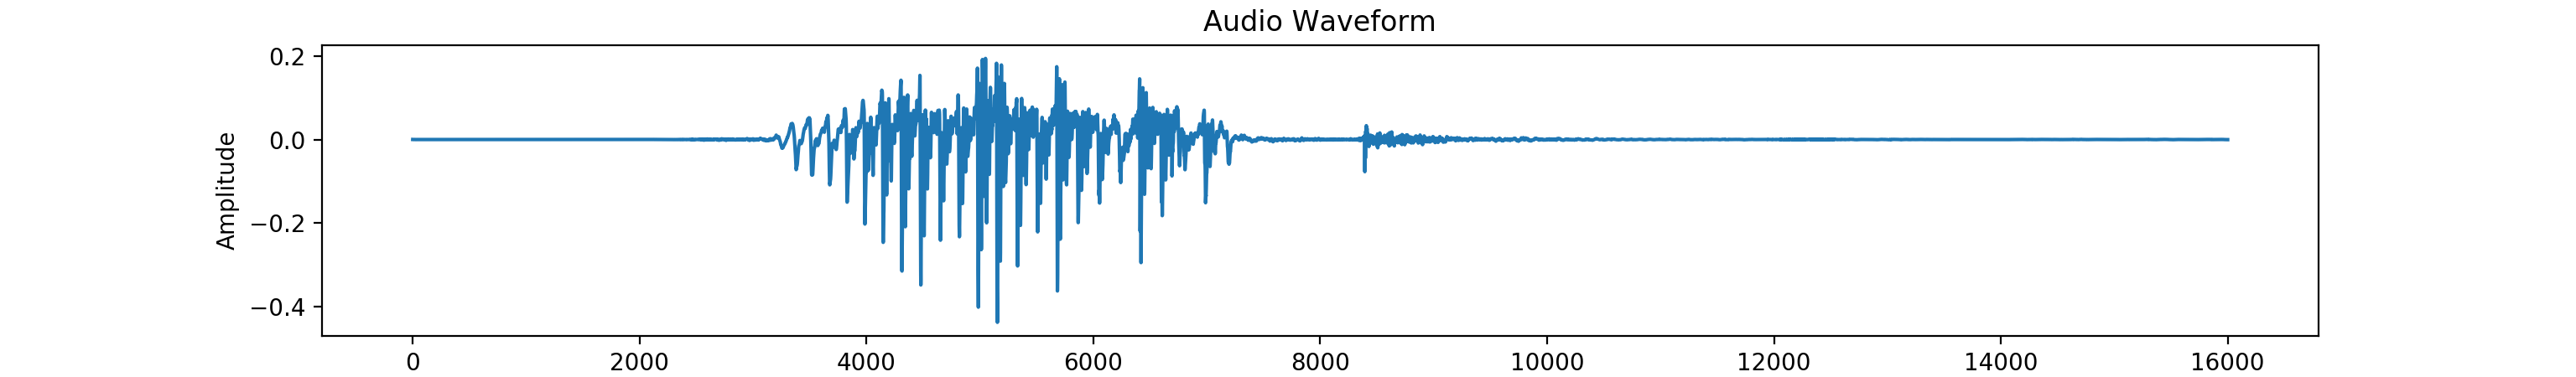
\includegraphics[width=\linewidth]{images/waveform-right}
    \caption{Audio waveform of utterance ``right''}
    \label{fig:wave_right}
  \end{subfigure}%
  \begin{subfigure}{.5\linewidth}
    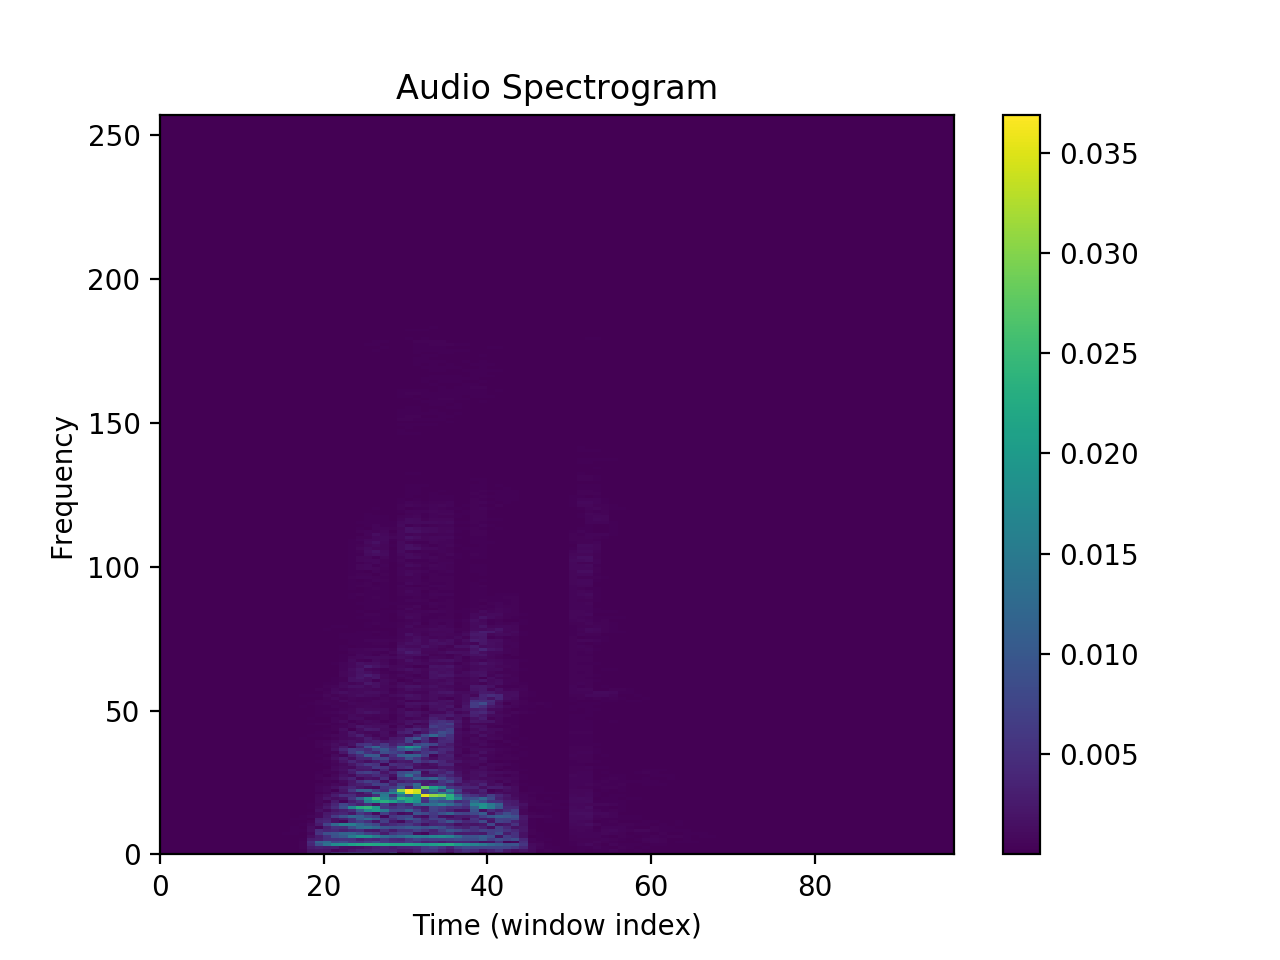
\includegraphics[width=\linewidth]{images/spectrogram-right}
    \caption{Audio spectrogram of utterance ``right''}
    \label{fig:spec_right}
  \end{subfigure}
  \caption{Representations of audio data}
\end{figure}

Model evaluation was also done with the use of spectrogram to
transform the audio waveform. The spectrogram computes the magnitude
of the short time fourier transform of the 1D audio waveform over a
short window of the data. The window of the transform passes over the
waveform through time with some stride. This representation of the
data provides the magnitude of different frequencies that compose the
audio waveform during the window that is under concideration. The
spectrogram of the utterence ``right'' is seen in figure
\ref{fig:spec_right}. The spectrogram shows that the waveform is
composed of large magnitudes of frequencies at the low end
corresponding to the word. For evaluation of the model without the use
of spectrograms as input data transformation, the audio waveform was
used keeping the sampling rate at 16KHz.

TODO: remove

Describe your dataset: how many training/validation/test examples do you have? Is there
any preprocessing you did? What about normalization or data augmentation? What is the
resolution of your images? How is your time-series data discretized? Include a citation on
where you obtained your dataset from. Depending on available space, show some examples
from your dataset. You should also talk about the features you used. If you extracted
features using Fourier transforms, word2vec, PCA,
ICA, etc. make sure to talk about it. Try to include examples of your data in the report
(e.g. include an image, show a waveform, etc.).



\section{ Methods }
As a simple baseline model, a simple multilayer convolutional neural
network (CNN) was evaluated[1]. The motivation behind a CNN network
architecture is to take advantage of the 2D nature of the spectrogram
of the sound wave. Since the spectorgram is two dimensional, a 2D
convolutional filter should be able to extract features from this
representation of the input. Coupled with this is the fairly
consistent size of the input audio waveform, and a CNN netwrok can
take the spectrogram of an entire speech utterance as an input
image. The specfic CNN model that was used for the baseline is a 4
layer CNN interleaved with 2x2 max pool layers. The convolutional
layers all implement 3x3 filter kernels and contain power of two
multiples of 16 filters per layer (The layers from 1 to 4 contain
16, 32, 64, 128 filters respectively. These are then followed by 2
fully connected layers and finally a softmax output layer. Also
evaluated are networks with time dimensional colvolutions feed to a
recurrent LSTM layer. These would correspond to the more traditional
recurrent speech recognition networks.

These two models are merged into a hybrid network taking the
advantages of both systems. At the end of the convolutional layers, we
are left with a time sequence of several frequency features for each
of the filter bank outputs. At this point, instead of performing a max
or average pooling step across all of the frequencies, we stack all of
the frequency and filter outputs for a point in time into a single
feature vector at that time point. This allow for keeping separation
between the frequency features for the output of each filter bank to
feed into the recurrent layers. The following is a fairly standard
multi-layer recurrent network. which feeds to a softmax output to
determine the command class.

The proposed network takes a batch of spectograms of audio data. Since
our data has been processed to all be of a fixed length at 16,000
samples, we can batch samples together to pass into our network for
efficiency. The input spectrogram contains 512 frequencies over 512
sample windows of the audio waveform. The audio windows for spectral
transformation have a stride of 160 pixels (or 10ms) of audio. This
generates an input data set of 512 freqencies over 97 time samples of
data. This feeds multiple 2D convolutional and max pooling layers.

The colvolutional layers successively perform 2D convolution on the
input. Following the convolution is a batch normalization layer to aid
in training. Before being fed into the next set of convolutional layer
there is a dropout layer to aid in reducing the variance of the
network. This is then fed into the activation layer which uses a
ReLU activation function. Finally, there is a max pooling step with a
2x2 window and a stride of 2 samples to produce the output of the
convolution layer. This set of layers are repeated with more filters
used in each layer. The convolutions will extract features in both the
time and frequncy domains and look for certain patterns in the
data. The max pool step in each layer provides some level of
invariance in both time and frequency to account for variations in the
speed that the speaker is speaking and also the pitch of the
speaker. The multiple layers will extract larger and larger features
in the data where individual sounds uttered can vary in both time and
frequency due to the use of the max polling layers to aid in
robustness.

The outputs of the convolutional portion of the network are then
flattened per time step and fed to one of more recurrent layers. These
recurrent layers perform sequential modelling of the input data from
the convolutions over time. The LSTM layers use a hyperbolic tangent
activation function. The recurrent activation function is the hard
sigmoid function.
These recurrent layers allow us to process
the audio data over time without needing to have access to the entire
sample at once. The advanatage here is that we can continually feed
data into the recurrent network as we get more audio data which
overcomes the main drawback of the fully connected or convolutional
only network architectures. Beyond that, as we get more audio data
over time, we can only keep a window of convolutional results and add
to it as we get more raw data. We don't need to keep all of the raw
data to process, but rather only enough that we can generate new
convolutional results as needed.

The output of the last LSTM layer passes into a fully connected layer
which generates a softmax output. The loss for the network is the
categorical loss function for single class selection based on one-hot
encoding.

TODO: Provide loss function as equation.


TODO: REMOVE

Describe your learning algorithms, proposed algorithm(s), or theoretical proof(s). Make
sure to include relevant mathematical notation. For example, you can include the loss function you are using. It is okay to use formulas from the lectures (online or in-class). For each algorithm, give a short description 
of how it works. Again, we are looking for your understanding of how these deep
learning algorithms work. Although the teaching staff probably know the algorithms, future
readers may not (reports will be posted on the class website). Additionally, if you are
using a niche or cutting-edge algorithm (anything else not covered in the class), you may want to explain your algorithm using 1/2
paragraphs. Note: Theory/algorithms projects may have an appendix showing extended
proofs (see Appendix section below).

\section{Experiments/Results/Discussion}

TODO: Remove

You should also give details about what (hyper)parameters you chose (e.g. why did you
use X learning rate for gradient descent, what was your mini-batch size and why) and how
you chose them. What your primary metrics are: accuracy, precision,
AUC, etc. Provide equations for the metrics if necessary. For results, you want to have a
mixture of tables and plots. If you are solving a classification problem, you should include a
confusion matrix or AUC/AUPRC curves. Include performance metrics such as precision,
recall, and accuracy. For regression problems, state the average error. You should have
both quantitative and qualitative results. To reiterate, you must have both quantitative
and qualitative results! If it applies: include visualizations of results, heatmaps,
examples of where your algorithm failed and a discussion of why certain algorithms failed
or succeeded. In addition, explain whether you think you have overfit to your training set
and what, if anything, you did to mitigate that. Make sure to discuss the figures/tables in
your main text throughout this section. Your plots should include legends, axis labels, and
have font sizes that are legible when printed.

\section{Conclusion/Future Work }
Summarize your report and reiterate key points. Which algorithms were the highestperforming?
Why do you think that some algorithms worked better than others? For
future work, if you had more time, more team members, or more computational resources,
what would you explore?

\section{Contributions}
The contributions section is not included in the 5 page limit. This section should describe
what each team member worked on and contributed to the project.

\section*{References}
This section should include citations for: (1) Any papers mentioned in the related work
section. (2) Papers describing algorithms that you used which were not covered in class.
(3) Code or libraries you downloaded and used. This includes libraries such as scikit-learn, Tensorflow, Pytorch, Keras etc. Acceptable formats include: MLA, APA, IEEE. If you
do not use one of these formats, each reference entry must include the following (preferably
in this order): author(s), title, conference/journal, publisher, year. If you are using TeX,
you can use any bibliography format which includes the items mentioned above. We are excluding
the references section from the page limit to encourage students to perform a thorough
literature review/related work section without being space-penalized if they include more
references. Any choice of citation style is acceptable
as long as you are consistent. 

\medskip
\small
[1] Alexander, J.A.\ \& Mozer, M.C.\ (1995) Template-based algorithms
for connectionist rule extraction. In G.\ Tesauro, D.S.\ Touretzky and
T.K.\ Leen (eds.), {\it Advances in Neural Information Processing
  Systems 7}, pp.\ 609--616. Cambridge, MA: MIT Press.

[2] Bower, J.M.\ \& Beeman, D.\ (1995) {\it The Book of GENESIS:
  Exploring Realistic Neural Models with the GEneral NEural SImulation
  System.}  New York: TELOS/Springer--Verlag.

[3] Hasselmo, M.E., Schnell, E.\ \& Barkai, E.\ (1995) Dynamics of
learning and recall at excitatory recurrent synapses and cholinergic
modulation in rat hippocampal region CA3. {\it Journal of
  Neuroscience} {\bf 15}(7):5249-5262.

\end{document}
